\documentclass{TIJMUjiaoanSY}
\pagestyle{empty}


\begin{document}


%课程名称
\kecheng{Linux系统概论}
%实验名称
\shiyan{实验2\ Linux图形界面的基本操作}
%教师姓名
\jiaoshi{伊现富}
%职称
\zhicheng{讲师}
%教学日期(格式:XXXX年XX月XX日XX时-XX时)
\riqi{2018年5月14日13:30-15:30}
%授课对象(格式:XXX系XXXX年级XX班(硕/本/专科))
\duixiang{生物医学工程学院2016级生信班(本)}
%实验人数
\renshu{28}
%实验类型
\leixing{验证型}
%实验分组
\fenzu{一人一机}
%学时数
\xueshi{2}
%教材版本
\jiaocai{Linux系统概论上机指南(自编教材)}


%教案首页
\firstHeader
\maketitle
\thispagestyle{empty}

\mudi{
\begin{itemize}
  \item 了解常见的Linux桌面环境。
  \item 掌握GNOME桌面环境的使用。
  \item 掌握文件浏览器的使用方法。
  \item 掌握桌面环境下管理用户和组的方法。
\end{itemize}
}

\fenpei{
\begin{itemize}
  \item (10')Linux用户界面:介绍Linux的两种用户界面——GUI和CLI,并对它们进行比较。
  \item (10')Linux桌面环境:介绍常见的Linux桌面环境,关联常见的Linux发行版和桌面环境。
  \item (80')实验操作:以CentOS发行版为例,练习GNOME桌面环境、文件浏览器的使用,学习桌面环境下用户和组的管理。
\end{itemize}
}

\cailiao{
\begin{itemize}
  \item 主要仪器:一台安装有CentOS的计算机。
\end{itemize}
}

\zhongdian{
\begin{itemize}
  \item 重点难点:GNOME桌面环境的使用,用户和组的管理。
  \item 解决策略:通过演示进行学习,通过练习熟练掌握。
\end{itemize}
}

\sikao{
\begin{itemize}
  \item 比较GUI和CLI这两种Linux的用户界面。
  \item 列举常见的Linux桌面环境。
  \item 列举常见的Linux发行版及其默认的桌面环境。
  \item 总结GNOME桌面环境的使用方法。
  \item 总结GNOME桌面环境下管理用户和组的方法。
\end{itemize}
}

\cankao{
\begin{itemize}
  \item Linux基础及应用习题解析与实验指导(第二版),谢蓉\ 编著。中国铁道出版社,2014。
\end{itemize}
}

\firstTail


%教案续页
\newpage
\otherHeader

\noindent
\begin{enumerate}
  \item Linux用户界面(10分钟)
    \begin{enumerate}
      \item 两种用户界面
	\begin{itemize}
	  \item 图形用户界面(Graphical User Interface,GUI):指采用图形方式显示的计算机操作用户界面。
	  \item 命令行界面(Command Line Interface,CLI):图形用户界面得到普及之前使用最为广泛的用户界面,它通常不支持鼠标,用户通过键盘输入指令,计算机接收到指令后,予以执行。
	\end{itemize}
      \item GUI vs. CLI\\
	\vspace*{-10pt}
\parpic[fr]{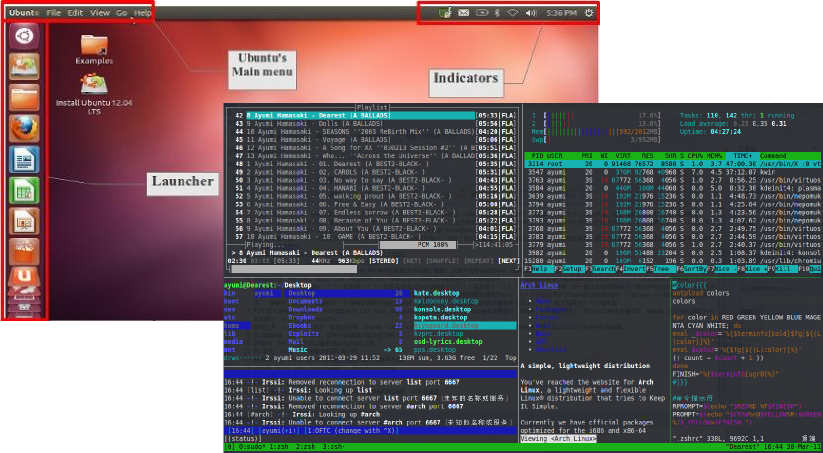
\includegraphics[width=8cm]{c1_gui_cli.png}}
	\textcolor{red}{Graphical user interfaces make easy tasks easier, while command line interfaces make difficult tasks possible.}
	\begin{itemize}
	  \item GUI对于用户来说在视觉上更易于接受
	  \item CLI没有GUI那么方便用户操作
	  \item CLI比GUI节约计算机系统的资源
	  \item 使用CLI往往比使用GUI的操作速度快
	\end{itemize}
    \end{enumerate}
  \item Linux桌面环境(10分钟)
    \begin{enumerate}
      \item 桌面环境\\
	一个桌面环境(Desktop environment,有时称为桌面管理器)为计算机提供一个图形用户界面(GUI)。这个名称来自桌面比拟,对应于早期的文字命令行界面(CLI)。一个典型的桌面环境提供图标、视窗、工具栏、文件夹、壁纸以及像拖放这样的能力。整体而言,桌面环境在设计和功能上的特性,赋予了它与众不同的外观和感觉。
      \item Linux桌面环境
	\begin{itemize}
	  \item GNOME:GNU网络对象模型环境(The GNU Network Object Model Environment),GNU计划的一部分,开放源码运动的一个重要组成部分。其目标是基于自由软件,为Unix及类Unix系统构造一个功能完善、操作简单以及界面友好的桌面环境。它是GNU计划的正式桌面。
	  \item KDE:一个国际性的自由软件社区,开发运行在Linux、BSD、Solaris、Microsoft Windows与Mac OS X等平台上的一系列跨平台应用程序。它最著名的产品是Plasma桌面,是许多Linux发布版的默认桌面环境。
	  \item Unity:Canonical公司为GNOME桌面环境所开发的图形用户界面,用于Ubuntu操作系统。Unity在Ubuntu 10.10上网本版中首次推出,最初是为了充分利用上网本有限的屏幕尺寸。不同于GNOME、KDE,Unity并非一个桌面包。
	  \item CDE:通用桌面环境(Common Desktop Environment),运行于Unix、基于Motif部件工具箱开发的商业桌面环境。
	  \item Xfce:一个在Unix与Unix-like操作系统上运行的桌面环境。Xfce的设计目的是“设计为可作为实际应用,快速加载及运行程序,并减少耗用系统资源”。
	  \item LXDE:Lightweight X11 Desktop Environment,是自由桌面环境,可在Unix以及Linux等POSIX兼容平台运行。LXDE项目旨在提供新的轻量、快速的桌面环境。LXDE重视实用性和轻巧性,并且尽力降低其所耗系统资源。
	  \item Enlightenment:常简称为E。0.17以前版本属于X窗口管理器,0.17版已经接近完整的桌面环境。而从0.19版开始,同时也是Wayland的合成管理器。
	  \item Cinnamon:Unix-like系统下的一个用户接口。是GNOME Shell的一个派生版本,最初是为Linux Mint所开发,其提供了如同GNOME 2般,易于使用的拟真接口。
	  \item MATE:由已经停止官方维护的GNOME 2源代码派生而来的桌面环境。


\otherTail
\newpage
\otherHeader

\parpic[fr]{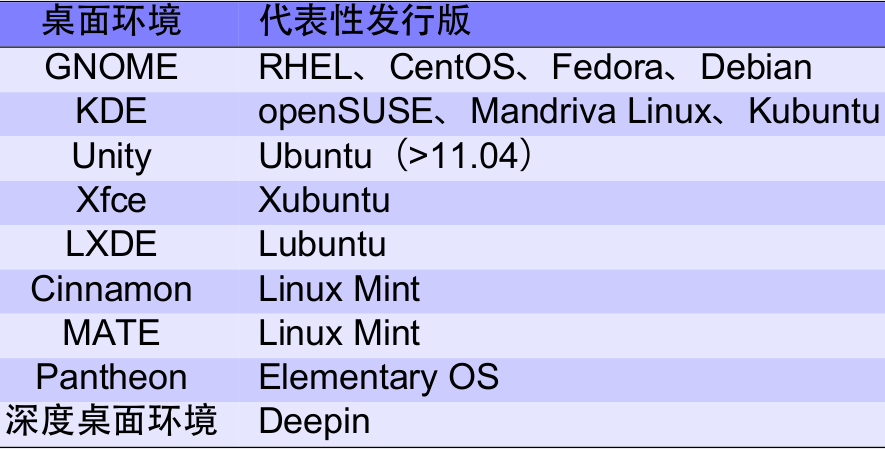
\includegraphics[width=9cm]{c1_distro_desktop.png}}
	  \item 深度桌面环境:Deepin Desktop Environment,基于HTML5和WebKit开发,主要由桌面、启动器、任务栏和深度控制中心组成。除深度控制中心前端使用QML技术,后端使用Go语言编写外,其余部分均为HTML5和WebKit实现。

	\end{itemize}
      \item Linux发行版与桌面环境
    \end{enumerate}
  \item 实验操作(75分钟)
    \begin{enumerate}
      \item 设置面板\textcolor{red}{(参考Windows中底部工作栏的设置方法)}
	\begin{itemize}
	  \item 设置底部面板可隐藏
	  \item 在顶部面板上添加、移动和删除对象
	\end{itemize}
      \item 设置桌面\textcolor{red}{(参考Windows中桌面的设置方法)}
	\begin{itemize}
	  \item 更改桌面背景
	  \item 设置屏幕保护程序
	  \item 设置桌面图标
	\end{itemize}
      \item 系统设置\textcolor{red}{(参考Windows中系统设置的方法)}
	\begin{itemize}
	  \item 设置主题
	  \item 增加启动项
	  \item 设置输入法
	\end{itemize}
      \item 使用文件浏览器\textcolor{red}{(参考Windows中文件浏览器的使用方法)}
	\begin{itemize}
	  \item 基本文件操作:新建、复制、重命名、……
	  \item 查看隐藏文件
	\end{itemize}
      \item 桌面环境下用户和组的管理\textcolor{red}{(注意每一步操作对配置文件的影响)}
	\begin{itemize}
	  \item 用户管理:新建、锁定、删除、……
	  \item 组管理:新建、修改、删除、……
	\end{itemize}
      \item 体验KDE、Unity、Xfce、LXDE等不同的桌面环境
    \end{enumerate}
\end{enumerate}


\otherTail


\end{document}

